\begin{figure*}[t]
    \centering
     \begin{subfigure}[t]{0.24\textwidth}
        \centering
        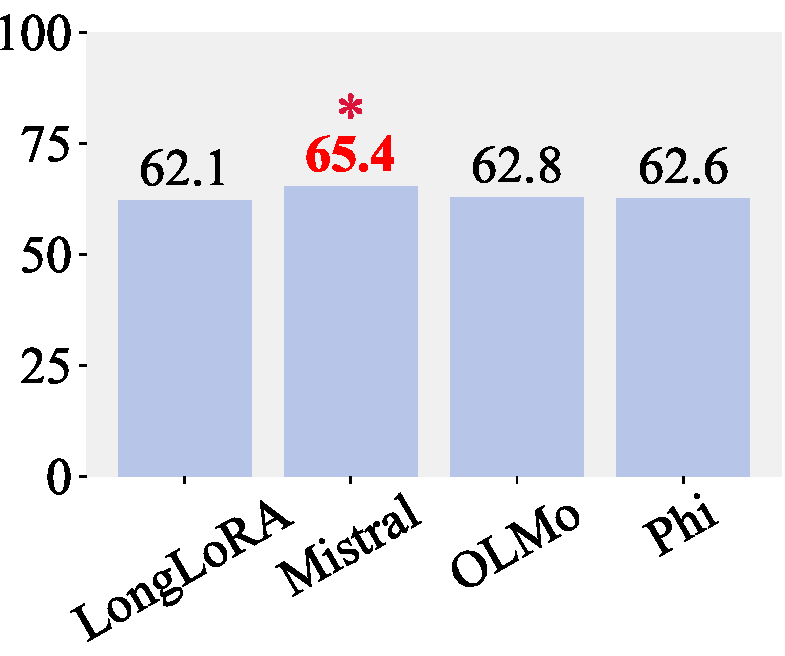
\includegraphics[width=\linewidth]{imgs/in_domain_avg/id_TableLlama.crop.pdf}
        \caption{TableLlama.}
    \end{subfigure}%
     \begin{subfigure}[t]{0.24\textwidth}
        \centering
        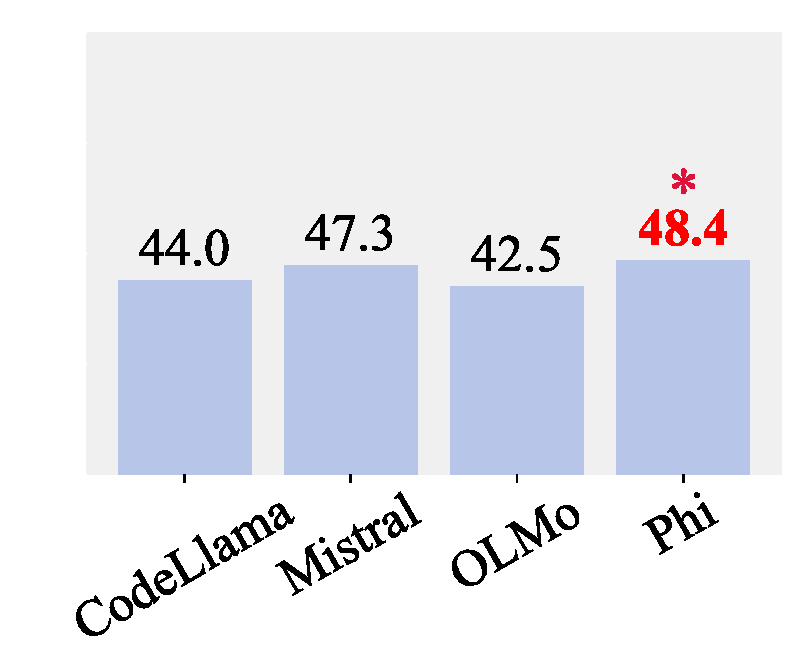
\includegraphics[width=\linewidth]{imgs/in_domain_avg/id_TableLLM.crop.pdf}
        \caption{TableLLM.}
    \end{subfigure}%
     \begin{subfigure}[t]{0.24\textwidth}
        \centering
        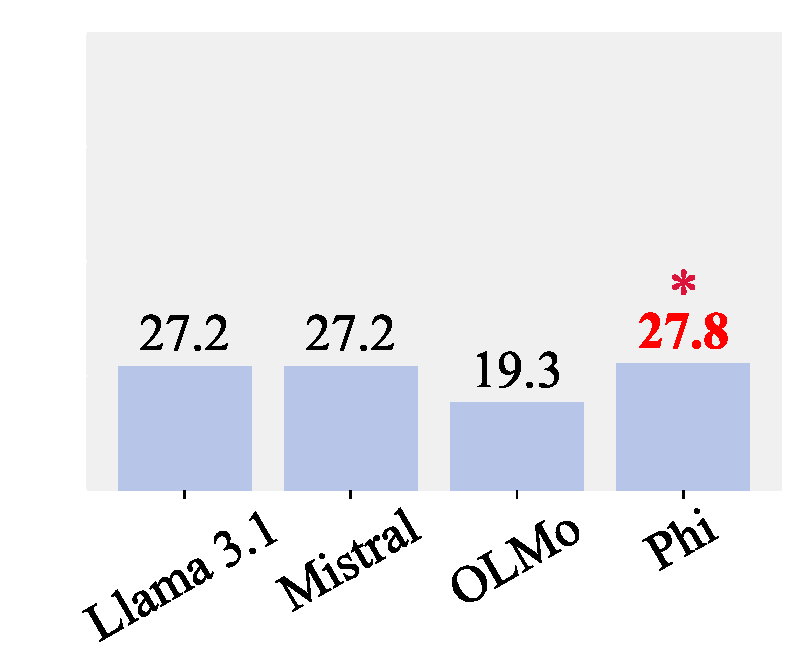
\includegraphics[width=\linewidth]{imgs/in_domain_avg/id_TableBench.crop.pdf}
        \caption{TableBench.}
    \end{subfigure}%
    \begin{subfigure}[t]{0.24\textwidth}
        \centering
        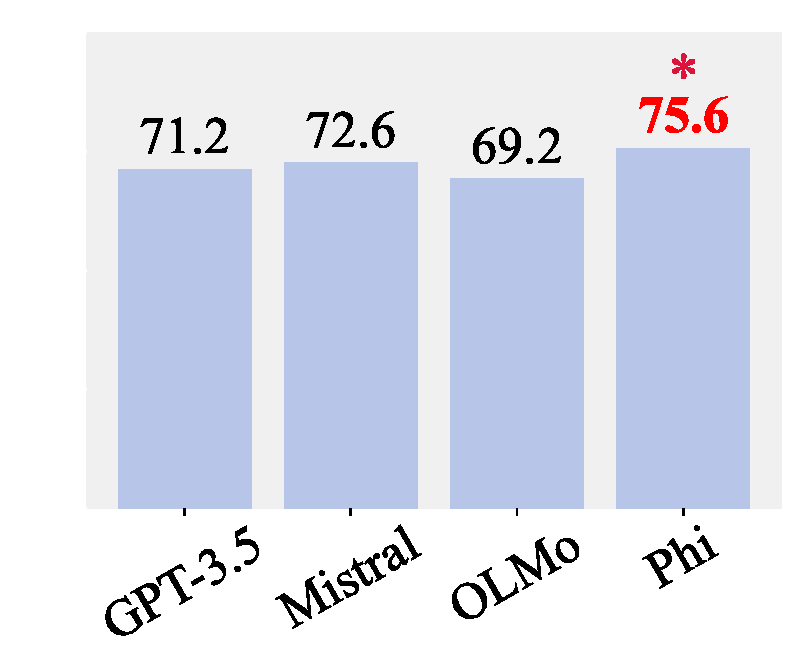
\includegraphics[width=\linewidth]{imgs/in_domain_avg/id_Table-GPT.crop.pdf}
        \caption{Table-GPT.}
    \end{subfigure}%

    \caption{Averaged in-domain performance (y-axis) between the models in existing works (the leftmost bar for each plot) versus our replications.
    Our replicated models achieve better in-domain results than the existing works.
    The detailed in-domain performance is reported in \Cref{app-sec: reimpl-compare}.
    }
    \label{fig:in-domain-perf}
\end{figure*}